
Zur effizienten Berechnung haben wir verwendet, dass die Multiplikation im Zeitbereich der Faltung im Frequenzbereich entspricht.
Anschliessend haben wir die schnelle Fourier-Transformation zur Berechnung der Bilder verwendet.
Die FFT berechnet jedoch eine Fourier-Reihe, welche im Kapitel~\ref{section:fourier-reihen} behandelt wurden.
Für Fourier-Reihen wurde vorausgesetzt, dass die Signale $2\pi$-periodisch und im Interval $\left[0, 2\pi\right)$ quadratintegrierbar sind.

Reale Signale sind aber nie periodisch.
Sie haben immer irgendwo einen Anfang $t_0$ und ein Ende $t_1$.
Abhilfe schafft hierbei der Periodisierungsoperator aus Definition~\ref{msa:peri}.
Sei $\tilde{x}(t)$ ein quadratintegrierbares Zeitsignal mit Träger $\left[t_0, t_1\right)$, dann ist
\[
	x(t) = \tilde{x}\left(2\pi\frac{t-t_0}{t_1-t_0}\right)
\]
eine affine Transformation auf das Interval $\left[0, 2\pi \right)$ und
\[
	\Peri x(t) = x( t \,\text{mod}\, 2\pi) \in L^2\left(\left[0, 2\pi \right)\right)
\]
ein $2\pi$-periodisches Signal, welches dieselbe Information beinhaltet, wie das ursprüngliche Signal $\tilde{x}(t)$.
Insbesondere rechnet die FFT immer mit diesem, äquivalenten Signal.
Erst darauf sind die Fourier-Reihen sinnvoll definiert und die gesammte Theorie funktioniert wie gewünscht.
Ausser, man beginnt, Signale miteinander zu falten.
Durch die Periodisierung des Ursprungssignals wurde das Signal vom ursprünglichen Interval $[t_0, t_1)$ auf ganz $\mathbb{R}$ erweitert.

\begin{figure}
	\centering
	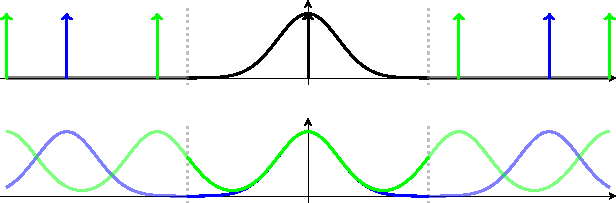
\includegraphics{papers/complex/images/cyclic_conv.pdf}
	\caption{Signal, gefaltet mit Dirac-Folgen unterschiedlicher Periode}
	\label{complex:cyclic-conv}
\end{figure}

Warum dies ein Problem ist, sei mit einem Beispiel illustriert.
In Abbildung~\ref{complex:cyclic-conv} ist ein Beispielsignal, welches mit einem Dirac gefaltet werden soll.
Dieser Dirac-Impuls sei nun aber periodisch.
Durch diese Fortsetzung überlappen die verschiedenen Signal-Kopien, falls am Rand nicht extra Platz gelassen wird.
Bei realen Signalen ist dies in der Regel nicht der Fall, die Aufzeichnung beginnt erst, wenn auch etwas interessantes passiert.

Es ist also wichtig, dem Signal vor der FFT extra Platz einzuräumen, sogenantes \emph{Signal Padding}.
Hierzu muss man sinnvolle Werte für das Signal ``erfinden''.
Dies kann auf verschiedene Arten geschehen.
Abbildung~\ref{complex:padding} zeigt die zwei meistverwendeten, Zero Padding und spiegeln an den Rändern.
\begin{figure}
	\centering
	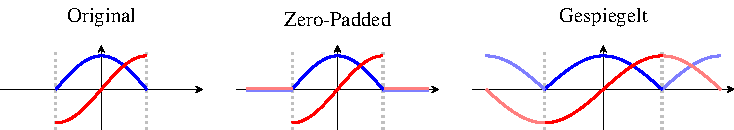
\includegraphics{papers/complex/images/signal_padding.pdf}
	\caption{Verschiedene Signal Padding-Optionen}
	\label{complex:padding}
\end{figure}

Die wohl einfachste Art ist das Auffüllen mit $0$.
Dies führt zu einem verschwinden des Signals am Rande, dafür müssen keine Sampels ``erfunden'' werden.
Diese Methode lässt sich auch gut begründen: wenn man das Signal nicht kennt, nehmen wir an, es sei $0$.
Zudem gibt sie am wenigsten zu tun.

Manchmal kann man das Signal auf geschicktere Art und Weise ergänzen, etwa durch extrapolation.
Gängig ist etwa das Signal an den Enden zu spiegeln.
Dadurch bleibt die Intensität des Signals am Rande erhalten.
Sinnvoll ist das jedoch nur, wenn man annehmen kann, dass das Signal auch eine entsprechende Symmetrie aufweist.
Selbst bei einem periodischen Signal tritt dadurch im Allgemeinen ein Phasensprung auf, da die Laufrichtung der Phase invertiert wird.

Anhand der beiden unteren Bilden in Abbildung~\ref{complex:padding} kann man sich leicht überzeugen, dass es keine ``richtige'' Art gibt, das Signal zu extrapollieren.
Gespiegelt resultiert in einer Phasen-Inversion, dafür tritt kein Phasen-Sprung auf.
Beim gespiegelten und komplex-konjugierten Signal ist es genau andersrum.

Man beachte, dass bei diesem Beispiel gespiegelt und konjugiert-komplex identisch ist mit der periodischen Fortsetzung.
Wären Real- und Imaginärteil im Original vertauscht, resultierte gespiegelt und komplex-konjugiert in korrekter Fortsetzung der Schwingung.

Dies soll verdeutlichen, dass es keine generell richtige Methode gibt, das Signal zu erweitern.
Falls die Randwerte wirklich wichtig sind, kann man versuchen, das Signal zu extrapolieren, etwa über eine Polynom-Aproximation.
Man sollte sich jedoch im Klaren sein, dass man gerade dabei ist, neue Signal-Werte zu erfinden.
Spiegeln ist deshalb meist die bevorzugte Wahl bei leistungsstarken Rechnern, mit Zero Padding macht man aber bestimmt nichts falsch.

Die Beispielsignale sind so gewählt, dass sie eine ganzzahlige Anzahl Perioden durchlaufen. 
Spiegeln an den Enden und komplex-konjugieren führt also zu einer korrekten Vortsetzung des Signals.
In den bisherigen Bildern wurde deshalb diese Methode gewählt, um Artefakte zu vermeiden.
Die Effekte können in den Abbildungen~\ref{complex:padding-none}~bis~\ref{complex:padding-sym-conj} betrachtet werden.
\begin{figure}
	\centering
	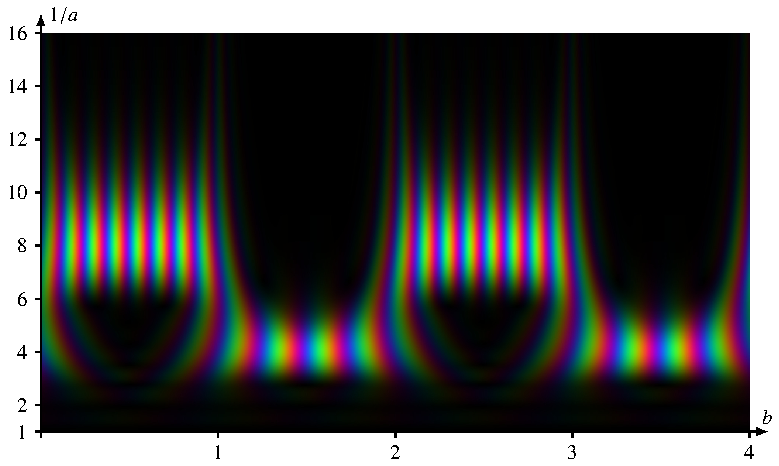
\includegraphics[width=\linewidth, keepaspectratio]{papers/complex/images/padding_none.pdf}
	\caption{Ohne Signal Padding} \label{complex:padding-none}
	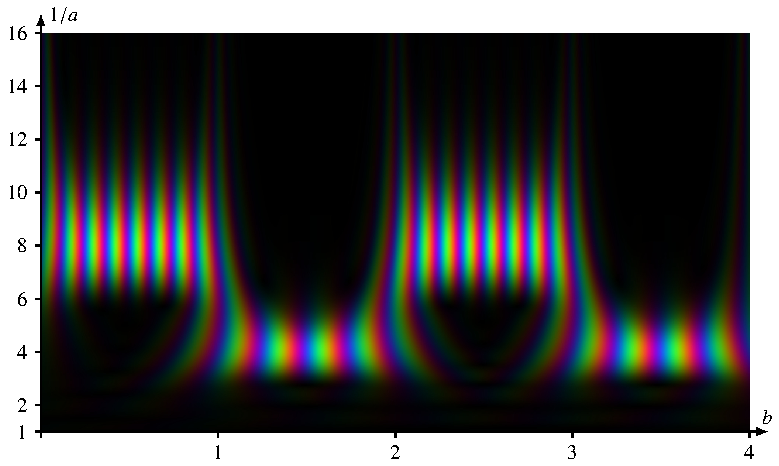
\includegraphics[width=\linewidth, keepaspectratio]{papers/complex/images/padding_zero.pdf}
	\caption{Zero Padded} \label{complex:padding-zero}
\end{figure}
\begin{figure}
	\centering
	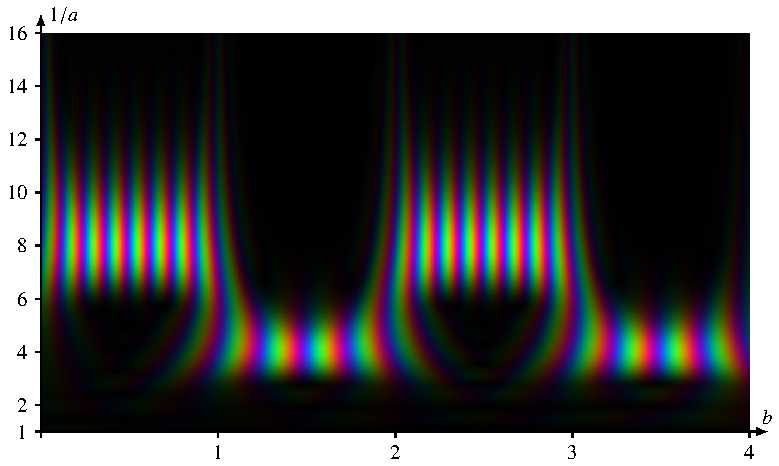
\includegraphics[width=\linewidth, keepaspectratio]{papers/complex/images/padding_sym.pdf}
	\caption{Signal an den Rändern gespiegelt} \label{complex:padding-sym}
	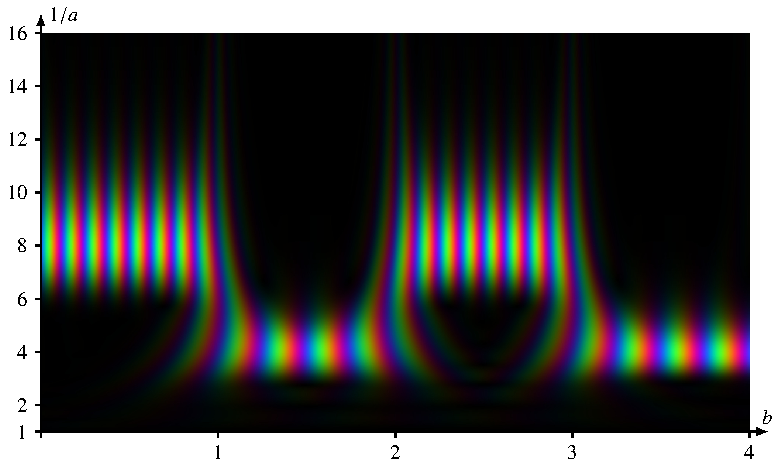
\includegraphics[width=\linewidth, keepaspectratio]{papers/complex/images/padding_sym_conj.pdf}
	\caption{Signal an den Rändern gespiegelt und komplex konjugiert} \label{complex:padding-sym-conj}
\end{figure}
